\documentclass{article}
\usepackage[utf8]{inputenc}
\usepackage{amsmath}
\usepackage{algorithm}
\usepackage{algorithmic}
\usepackage{subcaption}
\usepackage{natbib}
\usepackage{graphicx}
\usepackage{float}
\usepackage{listings}
\lstset{
    tabsize=2,
    basicstyle=\tiny
}

\title{Proyecto ADA}
\author{Mauricio Pinto, Jonathan Prieto, Alejandro Mamani}
\date{June 2020}
\url

\begin{document}
\maketitle
Repositorio: \href{https://github.com/jonathanprieto99/ProyectoADA}
\section{Pregunta 1 (Voraz)}
\subsection{Diseño}
Para obtener un matching (no necesariamente optimo), seguiremos el siguiente procedimiento:\\
 Sea $A_i$ un bloque de $A = A_1, A_2, ... A_n$ y $B_j$ un bloque de $B = B_1, B_2, ..., B_m$: 
 \begin{itemize}
     \item Se hará un matching del bloque $A_i$ con $B_j$ empezando con $i = 0$ y $j = 0$, e iremos incrementando a i y j en cada iteración hasta que lleguen a su máximo (el máximo de i es n y el máximo de j es m). Entonces, nuestro algoritmo tendría un tiempo de ejecución $O (max\{m,n\})$.
\end{itemize}
    Como ejemplo, pongamos a los siguientes bloques:\\
\begin{figure}
\centering
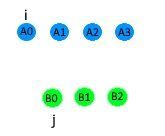
\includegraphics[scale=1]{ada1.jpeg}
\caption{El matching se hará entre $A_i$ y $B_j$, y se incrementarán sus valores.}
\end{figure}
\begin{figure}

    \centering
    
    \begin{subfigure}[b]{1\textwidth}
    \centering
    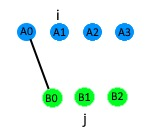
\includegraphics[]{ada2.jpeg}
    \caption{Paso 1: Matching e incrementación de los índices.}
    \label{fig:sub1}
    \end{subfigure}
    
    \begin{subfigure}[b]{1\textwidth}
    \centering
    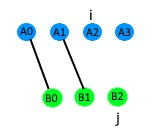
\includegraphics[]{ada3.jpeg}
    \caption{Paso 2: Matching e incrementación de los índices.}
    \label{fig:sub2}
    \end{subfigure}
    
    \begin{subfigure}[b]{1\textwidth}
    \centering
    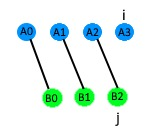
\includegraphics[]{ada4.jpeg}
    \caption{Paso 3: Matching e incrementación de los índices.}
    \label{fig:sub3}
    \end{subfigure}
    
\end{figure}
\begin{figure}

    \centering
    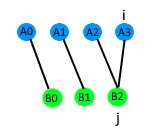
\includegraphics[]{ada5.jpeg}
    \caption{Paso 4: notar que ya que j alcanzó su valor máximo, no se incrementa. Se procede a hacer el matching de igual manera.}
    \label{fig:sub4}

\end{figure}

\newpage
Este procedimiento nos dejaría con el siguiente matching:
\[M = {(i_0, j_0)(i_1, j_1)(i_2, j_2)(i_3, j_2)}\]
\newpage
\subsection{Implementación}
\textbf{El pseudocodigo para nuestro algoritmo Greedy es el siguiente:}\\
\begin{algorithmic}

\STATE $result\gets 0$
\STATE $blocks\_A\gets get\_blocks (A)$
\STATE $blocks\_B\gets get\_blocks (B)$

\STATE $i\gets 0$
\STATE $j\gets 0$

\STATE $max\gets 0$

\STATE $n\gets blocks\_A.size()$
\STATE $m\gets blocks\_B.size()$

\IF {n $>$ m} 
        \STATE $max\gets m$
        \STATE $m\gets m-1$
\ELSE
        \STATE $max\gets m$
        \STATE $n\gets n-1$
\ENDIF 

\STATE $match\gets - -$
\STATE $weight\gets 0$

\WHILE{i $<$ max and j $<$ max}
\STATE $match.i\gets blocks\_A[i].index$
\STATE $match.j\gets blocks\_A[j].index$

\STATE $weight\gets weight + ((blocks\_A[i].j - blocks\_A[i].i + 1) / (blocks\_B[j].i + 1)$
\STATE $result.matching[-]\gets match$
\IF {i $<$ n} 
        \STATE $i\gets i+1$
\ENDIF
\IF {j $<$ m} 
        \STATE $j\gets j+1$
\ENDIF
\ENDWHILE
\STATE $result.weight\gets weight$
\RETURN result

\end{algorithmic}
\textit{La notación [-], representa un vector y [-]$<$- representa un push en un vector.}

\subsection{Análisis}
Para el análisis, omitiremos el tiempo de ejecución de los procedimientos $get\_blocks$.
Ya que todas las líneas previas y posteriores a la declaración while se ejecutan sólamente una vez, aportan un tiempo constante al tiempo total de ejecución. Sumaremos sus tiempos constantes en una constante $c$. Luego se itera incrementando a $i$ y $j$, hasta que alguno alcance el valor de $max$. Entonces, la línea que evalúa la condición del while aportaría al tiempo total de ejecución con:
\[T_w = c_wmax\]
donde $c_w$ representa al tiempo constante de ejecución de la instrucción. Luego, todas las $k$ líneas dentro de la declaración while se ejecutan $max - 1$ veces, por lo que aportan al tiempo total con:
\[T_k = \sum_{i=1}^{k} c_i(max-1)\]
donde $c_i$ representa la constante de tiempo que corresponde a la línea $i$ entre las $k$ líneas dentro de la expresión while. Por tanto, tenemos que el tiempo total de ejecución está dado por:
\[T_{total} = c_wmax + \sum_{i=1}^{k} c_i(max-1) + c\]
lo cual puede ser reducido a:
\[T_{total} = c_1max + d\]
donde $c_1$ es la suma entre $c_w$ y \(\sum_{i=1}^{k} c_i\), y d es la suma entre c y \(-\sum_{i=1}^{k} c_i\). Podemos asegurar que existen dos valores $max_0$ y $c_2$ tal que para todo valor de $max \geq max_0$ se cumpla que:
\[c_1max + d \leq c_2max\]
ya que si tomamos, por ejemplo, el caso $c_2 = 2c_1$, eventualmente $2c_1max$ será mayor o igual que $c_1max + d$ cuando $d \leq c_2max$, ya que $d$ es constante. Por tanto, podemos decir que:
\[T_{total} = O (max) = O (max((m, n))\]
\newpage

\section{Pregunta 2 (Recurrencia)}
\subsection{}
  \[
    \\OPT(i,j)=\left\{
                \begin{array}{ll}
                  \frac{A}{B} \xrightarrow[]{} \textrm {cuando i = j = 1}\\
                  \\
                  \frac{A_1}{ \sum_{i=1}^{n}B_{i} } \xrightarrow[]{} \textrm {cuando i = 1 y j $>$ 1}\\
                  \\
                  \frac{ \sum_{i=1}^{n}A_{i}} {B_1} \xrightarrow[]{} \textrm {cuando j = 1 y i $>$ 1}\\
                  \\
                  min(M_A(i,j), M_B(i,j))\xrightarrow[]{} \textrm {otros casos}\\
                
                \end{array}
              \right.
  \]
  
\begin{algorithmic}
\STATE $M_A(i,j)\gets min^{1}_{k=i-1}(OPT(K,j-1)+\frac {\sum_{k+1}^{i}{A_{i}}}{B_j} )$
\end{algorithmic}
\\
\begin{algorithmic}
\STATE $M_B(i,j)\gets min^{1}_{k=j-1}(OPT(i-1,K)+\frac {A_i}{\sum_{k+1}^{j}{B_{j}}})$
\end{algorithmic}


\newpage
\section {Pregunta 3 (Recursivo)}
\subsection{Diseño}
Para resolver el problema del matching mínimo de manera recursiva, se planteó el siguiente procedimiento:

Sean $i, j, k$ índices de los grupos de bloques $A$ y $B$, donde $A_i$ es un bloque de $A$ en la posición $i = A.size ()$, $B_i$ un bloque de $B$ en la posición $j = B.size ()$ y $A_k, B_K$ bloques de $B$ o $A$ en la posición $k$: La búsqueda del matching mínimo se dividirá en dos sub-procedimientos:
\begin{itemize}
    \item El primero donde $k$ itera sobre los bloques de $A$, desde $i - 1$ hasta $1$. En este caso (llamemosle (a)), se partirá el problema en dos subproblemas, uno con los bloques entre $A_{k+1}$ hasta $A_i$ y el bloque $B_j$, y el otro con los bloques restantes. Se decrementa a $k$ y se repite este proceso hasta $k = 1$. Se hará una llamada recursiva a cada subproblema del lado izquierdo, que contendrá bloques de $A_1$ hasta $A_k$ y bloques de $B_1$ hasta $B_{j-1}$, y al lado derecho que contendrá bloques de $A_{k+1}$ hasta $A_i$ y el bloque $B_j$. Se encontrará el peso minimo de la suma de los pesos de los matchings de ambos subproblemas. Nótese que para el subproblema del lado derecho siempre se tendrá un caso base, definido cuando $i = 1$, $j = 1$ o $i = j = 1$.
    \item El segundo donde $k$ itera sobre los bloques de $B$, desde $j - 1$ hasta $1$. En este caso (llamemosle (b)), se partirá el problema en dos subproblemas, uno con los bloques entre $B_{k+1}$ hasta $B_j$ y el bloque $A_i$, y el otro con los bloques restantes. Se decrementa a $k$ y se repite este proceso hasta $k = 1$. Se hará una llamada recursiva a cada subproblema del lado izquierdo, que contendrá bloques de $B_1$ hasta $B_k$ y bloques de $A_1$ hasta $A_{i-1}$, y al lado derecho que contendrá bloques de $B_{k+1}$ hasta $B_j$ y el bloque $A_i$. Se encontrará el peso minimo de la suma de los pesos de los matchings de ambos subproblemas. Nótese que para el subproblema del lado derecho siempre se tendrá un caso base, definido cuando $i = 1$, $j = 1$ o $i = j = 1$.
\end{itemize}
Luego, se compara el peso de ambos matchings encontrados y se retorna el de menor peso.\\
\newpage
Como ejemplo para visualizar la partición, pongamos a los siguientes bloques:\\

    \begin{figure}[H]{1\textwidth}
    \centering
    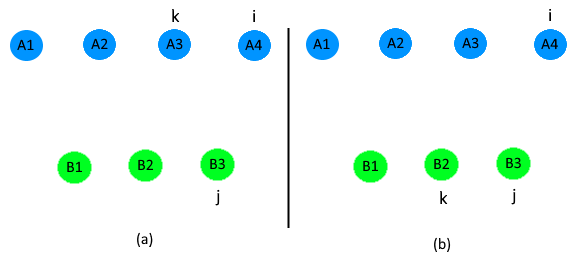
\includegraphics[]{ada13.png}
    \caption{Para el sub-procedimiento (a), k toma el valor de $i - 1$ y para el sub-procedimiento (b) toma el valor de $j - 1$.}
    \label{fig:sub1}
    \end{figure}
    
    \begin{figure}[H]{1\textwidth}
    \centering
    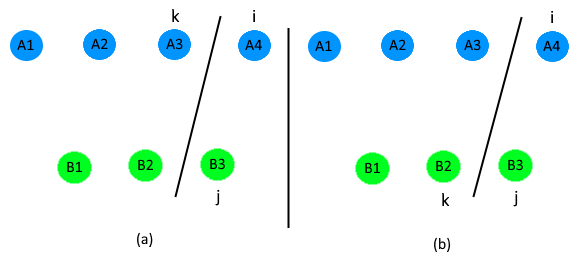
\includegraphics[]{ada14.png}
    \caption{Se hace la división del problema en dos subproblemas como se mencionó anteriormente. La línea negra representa la división.}
    \label{fig:sub2}
    \end{figure}
    
    \begin{figure}[H]{1\textwidth}
    \centering
    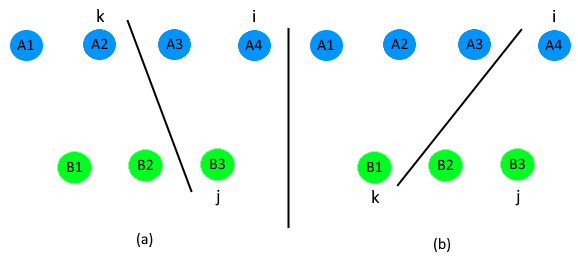
\includegraphics[]{ada15.png}
    \caption{A medida que los valores de $k$ disminuyen, se van haciendo distintas particiones. En caso de (b), $k$ llega a su valor mínimo.}
    \label{fig:sub3}
    \end{figure}
    
    \begin{figure}[H]{1\textwidth}
    \centering
    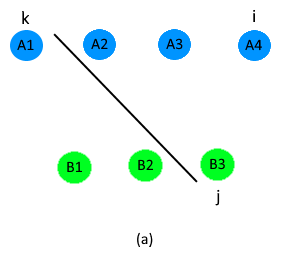
\includegraphics[]{ada16.png}
    \caption{Se hace la última partición en (a) y $k$ llega a su valor mínimo.}
    \label{fig:sub4}
    \end{figure}
\newpage    
\subsection{Implementación}
\textbf{El pseudocodigo para nuestro algoritmo Recursivo es el siguiente:}
\begin{algorithmic}

\STATE $min\_match\gets 0$

\STATE $i\gets A.size()-1$
\STATE $j\gets B.size()-1$

\STATE $min\_agrupaci{ó}n$
\STATE $min\_divici{ó}n$

\STATE $min\_agrupaci{ó}n.weight\gets INT\_MAX$
\STATE $min\_divici{ó}n.weight\gets INT\_MAX$

\IF {A.size() == 1 and B.size() == 1} 
        \STATE $match\gets - -$
        \STATE $match.i\gets A[0].index$
        \STATE $match.j\gets B[0].index$
        \STATE $min\_match.matching[-]\gets match$
        \STATE $min\_match.weight\gets (A[0].j - A[0].i + 1) / (B[0].j - B[0].i + 1)$
        \RETURN min\_match
\ENDIF 

\IF {A.size() == 1 and B.size() $>$ 1} 
        \STATE $sum\gets 0$
        \STATE $match\gets - -$
        \STATE $match.i\gets A[0].index$
        \FOR{it $<$ B.size()}
        \STATE $match.j\gets B[it].index$
        \STATE $min\_match.matching[-]\gets match$
        \STATE $sum\gets sum + (B[it].j - B[it].i + 1)$
        \ENDFOR
        \STATE $min\_match.weight\gets (A[0].j - A[0].i + 1) / sum$
        \RETURN min\_match
\ENDIF 

\IF {B.size() == 1 and A.size() $>$ 1} 
        \STATE $sum\gets 0$
        \STATE $match\gets - -$
        \STATE $match.j\gets B[0].index$
        \FOR{it = 0; it $<$ A.size()}
        \STATE $match.i\gets A[it].index$
        \STATE $min\_match.matching[-]\gets match$
        \STATE $sum\gets sum + (A[it].j - A[it].i + 1)$
        \ENDFOR
        \STATE $min\_match.weight\gets sum / (B[0].j - B[0].i + 1)$
        \RETURN min\_match
\ENDIF

\FOR{k = i - 1; k $\geq$ 0}
    \STATE $left\_A[-](A.begin(),A.begin()+k+1)$
    \STATE $right\_A[-](A.begin()+k+1,A.end())$
    
    \STATE $left\_B[-](B.begin(),B.end()-1)$
    \STATE $right\_B$
    \STATE $right\_B[-]\gets (B[B.size()-1])$
    
    \STATE $min\_left\gets opt\_soluci{ó}n(left\_A, left\_B)$
    \STATE $min\_right\gets opt\_soluci{ó}n(right\_A, right\_B)$
    
    \STATE $merge$
    
    \STATE $merge.matching\gets merge\_matchings(min\_left.matching, min\_right.matching)$
    \STATE $merge.weight\gets min\_left.weight+min\_right.weight$
    
    \IF{merge.weight $<$ min\_agrupaci{ó}n.weight}
        \STATE $min\_agrupaci{ó}n\gets merge$
    \ENDIF
\ENDFOR

\FOR{k = j - 1; k $\geq$ 0}
    \STATE $left\_A[-](A.begin(),A.end()-1)$
    \STATE $right\_A[-]\gets (A[A.size()-1])$
    
    \STATE $left\_B[-](B.begin(),B.begin()+k+1)$
    \STATE $right\_B[-](B.begin()+k+1,B.end())$
    
    \STATE $min\_left\gets opt\_soluci{ó}n(left\_A, left\_B)$
    \STATE $min\_right\gets opt\_soluci{ó}n(right\_A, right\_B)$
    
    \STATE $merge$
    
    \STATE $merge.matching\gets merge\_matchings(min\_left.matching, min\_right.matching)$
    \STATE $merge.weight\gets min\_left.weight+min\_right.weight$
    
    \IF{merge.weight $<$ min\_divici{ó}n.weight}
        \STATE $min\_divici{ó}n\gets merge$
    \ENDIF
\ENDFOR

\RETURN min\_agrupaci{ó}n.weight $<$ min\_divici{ó}n.weight ?  min\_agrupaci{ó}n : min\_divici{ó}n 

\end{algorithmic}
\textit{La notación [-], representa un vector y [-]$<$- representa un push en un vector.}\\

\subsection{Demostración del tiempo de ejecución}
T(m,n)=$\Omega$(2$^${max(m,n)})\\
T(m,n)$\geq${c $\times$ 2^{max(m,n)}}\\
T(m,n)=$\sum_{k=0}^{m-1}T(k,n-1)+\sum_{k=0}^{n-1}T(m-1,k)$\\
\textrm {Por inducción} \xrightarrow[]{} $T(m,n) \geq{c$\times$2^{max(m,n)}}$\\
\textrm {Caso Base} \xrightarrow[]{} m=0, n=0\\
\textrm {Paso inductivo:}\\
T(m,n)=2$^${(0,0)}=1\\
T(m,n)$\geq\sum_{k=0}^{n}2^{max(m,k)}$\\
T(m,n)$\geq2^{max(m,k)}$
T(m,n)$>\Omega(2^{max(m,n)})$

\newpage
\section {Pregunta 4 (Memoizado)}
\subsection{Diseño}
Para el algoritmo memoizado se usó el mismo diseño que el recursivo, teniendo como única diferencia la adición de una matriz donde se almacenan las respuestas de los subproblemas hallados. La posición M[i][j] almacena el matching para un subproblema cuyos arreglos de entrada $A$ y $B$ tienen tamaños $i$ y $j$, respectivamente. Dado que pueden existir soluciones diferentes para dos subproblemas con arreglos de bloques de tamaños iguales (ya que los subproblemas se definen por el tamaño de los arreglos de bloques y no los tamaños de los bloques en ellos, los cuales son determinantes para hallar el peso del matching), sólamente almacenaremos las soluciones de las llamadas recursivas a los subproblemas de la izquierda (ya que los de la derecha siempre formarán un caso base). \\
\textbf{El pseudocodigo para nuestro algoritmo Memorizado es el siguiente:}
\subsection{Implementación}
\begin{algorithmic}

\STATE $min\_match\gets 0$

\STATE $i\gets A.size()-1$
\STATE $j\gets B.size()-1$

\STATE $min\_agrupaci{ó}n$
\STATE $min\_divici{ó}n$

\STATE $min\_agrupaci{ó}n.weight\gets INT\_MAX$
\STATE $min\_divici{ó}n.weight\gets INT\_MAX$

\IF {left} 
        \IF{A.size() $<$= mem.size() - 1 and B.size() $<$= mem[0].size() - 1}
            \IF{mem[A.size()][B.size()].weight $\neq$ 0}
                \RETURN mem[A.size()][B.size()]
            \ENDIF
        \ENDIF
\ENDIF 

\IF {A.size() == 1 and B.size() == 1} 
        \STATE $match\gets - -$
        \STATE $match.i\gets A[0].index$
        \STATE $match.j\gets B[0].index$
        \STATE $min\_match.matching[-]\gets match$
        \STATE $min\_match.weight\gets (A[0].j - A[0].i + 1) / (B[0].j - B[0].i + 1)$
        \RETURN min\_match
\ENDIF 

\IF {A.size() == 1 and B.size() $>$ 1} 
        \STATE $sum\gets 0$
        \STATE $match\gets - -$
        \STATE $match.i\gets A[0].index$
        \FOR{it = 0; it $<$ B.size()}
        \STATE $match.j\gets B[it].index$
        \STATE $min\_match.matching[-]\gets match$
        \STATE $sum\gets sum + (B[it].j - B[it].i + 1)$
        \ENDFOR
        \STATE $min\_match.weight\gets (A[0].j - A[0].i + 1) / sum$
        \RETURN min\_match
\ENDIF 

\IF {B.size() == 1 and A.size() $>$ 1} 
        \STATE $sum\gets 0$
        \STATE $match\gets - -$
        \STATE $match.j\gets B[0].index$
        \FOR{it = 0; it $<$ A.size()}
        \STATE $match.i\gets A[it].index$
        \STATE $min\_match.matching[-]\gets match$
        \STATE $sum\gets sum + (A[it].j - A[it].i + 1)$
        \ENDFOR
        \STATE $min\_match.weight\gets sum / (B[0].j - B[0].i + 1)$
        \RETURN min\_match
\ENDIF

\FOR{k = i - 1; k $\geq$ 0}
    \STATE $left\_A[-](A.begin(),A.begin()+k+1)$
    \STATE $right\_A[-](A.begin()+k+1,A.end())$
    
    \STATE $left\_B[-](B.begin(),B.end()-1)$
    \STATE $right\_B$
    \STATE $right\_B[-]\gets (B[B.size()-1])$
    
    \STATE $min\_left\gets opt\_soluci{ó}n(left\_A, left\_B)$
    \STATE $min\_right\gets opt\_soluci{ó}n(right\_A, right\_B)$
    
    \STATE $merge$
    
    \STATE $merge.matching\gets merge\_matchings(min\_left.matching, min\_right.matching)$
    \STATE $merge.weight\gets min\_left.weight+min\_right.weight$
    
    \IF{merge.weight $<$ min\_agrupaci{ó}n.weight}
        \STATE $min\_agrupaci{ó}n\gets merge$
    \ENDIF
    
    \STATE $mem[left\_A.size()][left\_B.size()]\gets min\_left$
    
\ENDFOR

\FOR{k = j - 1; k $\geq$ 0}
    \STATE $left\_A[-](A.begin(),A.end()-1)$
    \STATE $right\_A[-]\gets (A[A.size()-1])$
    
    \STATE $left\_B[-](B.begin(),B.begin()+k+1)$
    \STATE $right\_B[-](B.begin()+k+1,B.end())$
    
    \STATE $min\_left\gets opt\_soluci{ó}n(left\_A, left\_B)$
    \STATE $min\_right\gets opt\_soluci{ó}n(right\_A, right\_B)$
    
    \STATE $merge$
    
    \STATE $merge.matching\gets merge\_matchings(min\_left.matching, min\_right.matching)$
    \STATE $merge.weight\gets min\_left.weight+min\_right.weight$
    
    \IF{merge.weight $<$ min\_divici{ó}n.weight}
        \STATE $min\_divici{ó}n\gets merge$
    \ENDIF
    
    \STATE $mem[left\_A.size()][left\_B.size()]\gets min\_left$
    
\ENDFOR

\RETURN min\_agrupaci{ó}n.weight $<$ min\_divici{ó}n.weight ?  min\_agrupaci{ó}n : min\_divici{ó}n 

\end{algorithmic}
\textit{La notación [-], representa un vector y [-]$<$- representa un push en un vector.}\\

\subsection{Demostración del tiempo de ejecución}
T(m,n)=O(m,n)\\
C(m,n)$\geq${T(m,n)\geq{0}}\\
\textrm {Tenemos} \xrightarrow[]{} $T(m,n) =\sum_{k=0}^{m-1}T(k,n-1)+\sum_{k=0}^{n-1}T(m-1,k)$\\
\textrm {Tomaremos que el tiempo para resolver los subproblemas es constante}\\
K=\ n{ú}mero de problemas $\times$ tiempo\\
\textrm {Tendriamos:} \xrightarrow[]{} $k\times T(m-1,n-1)+k\times T(m-1,n-1)$\\
$=K\times 2(T(m-1,n-1))$\\
$=K\times 2C(m,n)$\\
$C(m,n)\geq{O(m,n)}=T(m,n)$\\

\newpage
\section{Anexos}
\subsection{Código en C++ del archivo min\_matching.cpp}
\begin{lstlisting}
#include <iostream>
#include <vector>
#include <climits>
#include <cstdlib>

using namespace std;

struct Pair {
    float i;
    float j;
    int index;
};

struct Matching {
    vector<Pair> matching;
    float weight;
};

/* Prototipos */
vector<Pair> get_blocks (vector<int>);
Matching greedy_matching (vector<int>, vector<int>);
Matching min_matching_recursive (vector<int>, vector<int>);
Matching min_matching_memoized (vector<int>, vector<int>);
Matching opt_solution (vector<Pair>, vector<Pair>);
Matchin opt_solution_mem (vector<Pair>, vector<Pair>, bool left);
vector<Pair> merge_matchings (vector<Pair>, vector<Pair>);
vector<int> string_to_vector (string);
void print_matching (Matching);

/* Matriz donde se almacenan soluciones a subproblemas */
vector<vector<Matching>> mem;

/* Funcion que genera los bloques para un vector. Recorre todo el vector
 * Generando bloques, por lo que tiene un tiempo de ejecucion de O(n) */
vector<Pair> get_blocks (vector<int> A) {
    vector<Pair> blocks;
    bool flag = false;
    Pair block;
    for (int i = 0; i < A.size (); i++) {
        block.index = blocks.size ();
        if (A[i] == 1) {
            if (!flag) {
                flag = true;
                block.i = i;
            }
            if (i == A.size () - 1) {
                    block.j = i;
                    blocks.push_back (block);
            }

        }
        else if (A[i] == 0) {
            if (flag) {
                flag = false;
                block.j = i - 1;
                blocks.push_back (block);
            }
        }
    }
    return blocks;
}

/*Genera un matching agrupando elementos de A y B uno por uno, y haciendo
 * agrupaciones y divisiones cuando uno de estos llega a su limite. Ya que 
 * siempre se recorrera el vector de bloques de mayor cantidad de elementos, 
 * tiene un tiempo de ejecucion de O(max{m, n})*/
Matching greedy_matching (vector<int> A, vector<int> B) {
    Matching result;

    vector<Pair> blocks_A = get_blocks (A);
    vector<Pair> blocks_B = get_blocks (B);

    int i = 0, j = 0;
    int n = blocks_A.size ();
    int m = blocks_B.size ();
    if (n == 0 or m == 0) {
        cout << "Error: No hay bloques en uno de los vectores" << endl;
        exit (1);
    }

    int max;
    if (n > m) {
        max = n;
        m -=1;
    }
    else {
        max = m;
        n -=1;
    }
    Pair match;
    float weight = 0;
    while (i < max && j < max) {
        match.i = blocks_A[i].index;
        match.j = blocks_B[j].index;
        weight += (blocks_A[i].j - blocks_A[i].i + 1) / (blocks_B[j].j - blocks_B[j].i + 1);
        result.matching.push_back (match);

        if (i < n)
            i++;
        if (j < m)
            j++;
    }
    result.weight = weight;
    return result;
}

/* Genera bloques para los vectores */
Matching min_matching_recursive (vector<int> A, vector<int> B) {
    vector<Pair> result;

    vector<Pair> blocks_A = get_blocks (A);
    vector<Pair> blocks_B = get_blocks (B);

    Matching min_matching = opt_solution (blocks_A, blocks_B);

    return min_matching;
}

Matching opt_solution (vector<Pair> A, vector<Pair> B) {
    Matching min_match;
    int i = A.size () - 1;
    int j = B.size () - 1;
    Matching min_agrupacion;
    Matching min_division;

    min_agrupacion.weight = INT_MAX;
    min_division.weight = INT_MAX;

    if (A.size () == 1 and B.size () == 1) {
        Pair match;
        match.i = A[0].index;
        match.j = B[0].index;
        min_match.matching.push_back (match);
        min_match.weight = (A[0].j - A[0].i + 1) / (B[0].j - B[0].i + 1);
        return min_match;
    }

    if (A.size () == 1 and B.size () > 1) {
        Pair match;
        float sum = 0;
        match.i = A[0].index;
        for (int it = 0; it < B.size (); it++) {
            match.j = B[it].index;
            min_match.matching.push_back (match);
            sum += B[it].j - B[it].i + 1;
        }
        min_match.weight = (A[0].j - A[0].i + 1) / sum;
        return min_match;
    }
    if (B.size () == 1 and A.size () > 1){
        Pair match;
        float sum = 0;
        match.j = B[0].index;
        for (int it = 0; it < A.size (); it++){
            match.i = A[it].index;
            min_match.matching.push_back (match);
            sum += A[it].j - A[it].i + 1;
        }
        min_match.weight = sum / (B[0].j - B[0].i + 1);
        return min_match;
    }

    for (int k = i - 1; k >= 0; k--) {
        vector<Pair> left_A (A.begin (), A.begin () + k + 1);
        vector<Pair> right_A (A.begin () + k + 1, A.end ());

        vector<Pair> left_B (B.begin (), B.end () - 1);
        vector<Pair> right_B; right_B.push_back (B[B.size () - 1]);

        Matching min_left = opt_solution (left_A, left_B);
        Matching min_right = opt_solution (right_A, right_B);

        Matching merge;
        merge.matching = merge_matchings (min_left.matching, min_right.matching);
        merge.weight = min_left.weight + min_right.weight;
        if (merge.weight < min_agrupacion.weight)
            min_agrupacion = merge;
        print_matching (merge);
    }
    for (int k = j - 1; k >= 0; k--) {
        vector<Pair> left_A (A.begin (), A.end () - 1);
        vector<Pair> right_A; right_A.push_back (A[A.size () - 1]);

        vector<Pair> left_B (B.begin (), B.begin () + k + 1);
        vector<Pair> right_B (B.begin () + k + 1, B.end ());

        Matching min_left = opt_solution (left_A, left_B);
        Matching min_right = opt_solution (right_A, right_B);

        Matching merge;
        merge.matching = merge_matchings (min_left.matching, min_right.matching);
        merge.weight = min_left.weight + min_right.weight;
        if (merge.weight < min_division.weight)
            min_division = merge;
        print_matching (merge);
    }

    return min_agrupacion.weight < min_division.weight ? min_agrupacion : min_division;
}

vector<Pair> merge_matchings (vector<Pair> left, vector<Pair> right) {
    for (int i = 0; i < right.size (); i++)
        left.push_back (right[i]);
    return left;
}

Matching min_matching_memoized (vector<int> A, vector<int> B) {
    vector<Pair> result;

    vector<Pair> blocks_A = get_blocks (A);
    vector<Pair> blocks_B = get_blocks (B);

    if (blocks_A.size () == 0 or blocks_B.size () == 0) {
        cerr << "Vector sin bloques introducido." << endl;
    }

    mem.resize (blocks_A.size ());
    for (int i = 0; i < blocks_A.size (); i++)
                mem[i].resize (blocks_B.size ());

    Matching min_matching = opt_solution_mem (blocks_A, blocks_B, false);

    return min_matching;
}

Matching opt_solution_mem (vector<Pair> A, vector<Pair> B, bool left) {
    Matching min_match;
    int i = A.size () - 1;
    int j = B.size () - 1;
    Matching min_agrupacion;
    Matching min_division;

    min_agrupacion.weight = INT_MAX;
    min_division.weight = INT_MAX;
    if (left) {
        if (A.size () <= mem.size () - 1 and B.size () <= mem[0].size () - 1) {
            if (mem[A.size ()][B.size ()].weight != 0) {
                return mem[A.size ()][B.size ()];
            }
        }
    }
    if (A.size () == 1 and B.size () == 1) {
        Pair match;
                match.i = A[0].index;
                match.j = B[0].index;
                min_match.matching.push_back (match);
                min_match.weight = (A[0].j - A[0].i + 1) / (B[0].j - B[0].i + 1);
                return min_match;
    }

    if (A.size () == 1 and B.size () > 1) {
        Pair match;
                float sum = 0;
                match.i = A[0].index;
                for (int it = 0; it < B.size (); it++) {
                        match.j = B[it].index;
                        min_match.matching.push_back (match);
                        sum += B[it].j - B[it].i + 1;
                }
                min_match.weight = (A[0].j - A[0].i + 1) / sum;
                return min_match;
    }

    if (B.size () == 1 and A.size () > 1){
        Pair match;
                float sum = 0;
                match.j = B[0].index;
                for (int it = 0; it < A.size (); it++){
                        match.i = A[it].index;
                        min_match.matching.push_back (match);
                        sum += A[it].j - A[it].i + 1;
                }
                min_match.weight = sum / (B[0].j - B[0].i + 1);
                return min_match;
    }

    for (int k = i - 1; k >= 0; k--) {
        vector<Pair> left_A (A.begin (), A.begin () + k + 1);
        vector<Pair> right_A (A.begin () + k + 1, A.end ());

        vector<Pair> left_B (B.begin (), B.end () - 1);
        vector<Pair> right_B; right_B.push_back (B[B.size () - 1]);

        Matching min_left = opt_solution_mem (left_A, left_B, true);
        Matching min_right = opt_solution_mem (right_A, right_B, false);

        Matching merge;
        merge.matching = merge_matchings (min_left.matching, min_right.matching);
        merge.weight = min_left.weight + min_right.weight;
        if (merge.weight < min_agrupacion.weight)
            min_agrupacion = merge;
        /*for (int h = 0; h < merge.matching.size (); h++)
            {
                    cout << "(" << merge.matching[h].i << "," << merge.matching[h].j << ")" << " ";
            }
        cout << merge.weight << endl;*/
        print_matching (merge);
        mem[left_A.size ()][left_B.size ()] = min_left;
    }
    for (int k = j - 1; k >= 0; k--) {
        vector<Pair> left_A (A.begin (), A.end () - 1);
        vector<Pair> right_A; right_A.push_back (A[A.size () - 1]);

        vector<Pair> left_B (B.begin (), B.begin () + k + 1);
        vector<Pair> right_B (B.begin () + k + 1, B.end ());

        Matching min_left = opt_solution_mem (left_A, left_B, true);
        Matching min_right = opt_solution_mem (right_A, right_B, false);

        Matching merge;
        merge.matching = merge_matchings (min_left.matching, min_right.matching);
        merge.weight = min_left.weight + min_right.weight;
        if (merge.weight < min_division.weight)
            min_division = merge;
        /*for (int h = 0; h < merge.matching.size (); h++)
            {
                    cout << "(" << merge.matching[h].i << "," << merge.matching[h].j << ")" << " ";
            }
        cout << merge.weight << endl;*/
        print_matching (merge);
        mem[left_A.size ()][left_B.size ()] = min_left;
    }

    return min_agrupacion.weight < min_division.weight ? min_agrupacion : min_division;
}

void print_matching (Matching result) {
    cout << "Matching: ";
        for (int i = 0; i < result.matching.size (); i++)
        {
                cout << "(" << result.matching[i].i << "," << result.matching[i].j << ")" << " ";
        }
        cout << endl << "Weight: " << result.weight << endl;
}

vector<int> string_to_vector (string str) {
    vector<int> result;
    for (int i = 0; i < str.length (); i++) {
        int value = str[i] - '0';
        if (value != 0 and value != 1){
            cout << "Error: Arreglo con valores no validos." << endl;
            vector<int> vacio;
            return vacio;
        }
        result.push_back (value);
    }
    return result;
}

int main () {
    vector<int> A;
    vector<int> B;
    while (true) {
        while (true) {
            string str_A, str_B;
            do {
                cout << "Ingrese arreglo A: ";
                cin >> str_A;
                if (str_A.length () == 0)
                    cout << "Arreglo vacio" << endl;
            } while (str_A.length () == 0);

            do {
                cout << "Ingrese Arreglo B: ";
                cin >> str_B;
                if (str_B.length () == 0)
                    cout << "Arreglo vacio" << endl;
            } while (str_B.length () == 0);
            if (str_A.length() == str_B.length ()) {
                A = string_to_vector (str_A);
                    B = string_to_vector (str_B);
                if (A.size () == 0 or  B.size () == 0)
                    cout << "Se ha ingresado un arreglo vacio" << endl;
                else
                    break;
            }
            else {
                cout << "Arreglos de tamanos distintos. Ingrese nuevamente" << endl;
            }

        }

       Matching result;
        int option;
        bool new_vector = false;
        cout << "[1] Matching Voraz" << endl;
        cout << "[2] Matching Minimo Recursivo" << endl;
        cout << "[3] Matching Minimo Memoizado" << endl;
        cout << "[4] Ingresar Nuevo Vector" << endl;
        cout << "[0] Salir" << endl;
        while (!new_vector) {
            cout << "Ingrese el algoritmo a utilizar: ";
            cin >> option;
            switch (option) {
                case 0:
                    return 0;
                case 1: ;
                    result = greedy_matching (A, B);
                    cout << "resultado" << endl;
                    print_matching (result);
                    break;
                case 2: ;
                    result = min_matching_recursive (A, B);
                    cout << "resultado" << endl;
                    print_matching (result);
                    break;
                case 3: ;
                    result = min_matching_memoized (A, B);
                    cout << "resultado" << endl;
                    print_matching (result);
                    break;
                case 4: ;
                    new_vector = true;
                    break;
                default:
                    cout << "No existe la opcion " << option << endl;

            }
        }
    }
}

\end{lstlisting}

\end{document}